\documentclass[10pt,a4paper]{article}\usepackage[]{graphicx}\usepackage[]{color}
%% maxwidth is the original width if it is less than linewidth
%% otherwise use linewidth (to make sure the graphics do not exceed the margin)
\makeatletter
\def\maxwidth{ %
  \ifdim\Gin@nat@width>\linewidth
    \linewidth
  \else
    \Gin@nat@width
  \fi
}
\makeatother

\definecolor{fgcolor}{rgb}{0.345, 0.345, 0.345}
\newcommand{\hlnum}[1]{\textcolor[rgb]{0.686,0.059,0.569}{#1}}%
\newcommand{\hlstr}[1]{\textcolor[rgb]{0.192,0.494,0.8}{#1}}%
\newcommand{\hlcom}[1]{\textcolor[rgb]{0.678,0.584,0.686}{\textit{#1}}}%
\newcommand{\hlopt}[1]{\textcolor[rgb]{0,0,0}{#1}}%
\newcommand{\hlstd}[1]{\textcolor[rgb]{0.345,0.345,0.345}{#1}}%
\newcommand{\hlkwa}[1]{\textcolor[rgb]{0.161,0.373,0.58}{\textbf{#1}}}%
\newcommand{\hlkwb}[1]{\textcolor[rgb]{0.69,0.353,0.396}{#1}}%
\newcommand{\hlkwc}[1]{\textcolor[rgb]{0.333,0.667,0.333}{#1}}%
\newcommand{\hlkwd}[1]{\textcolor[rgb]{0.737,0.353,0.396}{\textbf{#1}}}%

\usepackage{framed}
\makeatletter
\newenvironment{kframe}{%
 \def\at@end@of@kframe{}%
 \ifinner\ifhmode%
  \def\at@end@of@kframe{\end{minipage}}%
  \begin{minipage}{\columnwidth}%
 \fi\fi%
 \def\FrameCommand##1{\hskip\@totalleftmargin \hskip-\fboxsep
 \colorbox{shadecolor}{##1}\hskip-\fboxsep
     % There is no \\@totalrightmargin, so:
     \hskip-\linewidth \hskip-\@totalleftmargin \hskip\columnwidth}%
 \MakeFramed {\advance\hsize-\width
   \@totalleftmargin\z@ \linewidth\hsize
   \@setminipage}}%
 {\par\unskip\endMakeFramed%
 \at@end@of@kframe}
\makeatother

\definecolor{shadecolor}{rgb}{.97, .97, .97}
\definecolor{messagecolor}{rgb}{0, 0, 0}
\definecolor{warningcolor}{rgb}{1, 0, 1}
\definecolor{errorcolor}{rgb}{1, 0, 0}
\newenvironment{knitrout}{}{} % an empty environment to be redefined in TeX

\usepackage{alltt}

\usepackage[T1]{fontenc}
\usepackage[polish]{babel}
\usepackage[cp1250]{inputenc}
\usepackage{amsmath}
\usepackage{amsfonts}
\usepackage{graphicx}
\usepackage{setspace}
\usepackage{savesym}
\savesymbol{arc}
\usepackage{color}
\usepackage{xcolor}
\usepackage{pict2e}
\usepackage{epstopdf}
\usepackage{geometry}

\newgeometry{tmargin=1cm, bmargin=1cm, lmargin=1cm, rmargin=1cm}
\pagestyle{empty}
\linespread{1.2}
\IfFileExists{upquote.sty}{\usepackage{upquote}}{}

\begin{document}

\section*{\centering BIOSTATYSTYKA - LABORATORIUM 1}

\begin{knitrout}
\definecolor{shadecolor}{rgb}{0.969, 0.969, 0.969}\color{fgcolor}\begin{kframe}
\begin{alltt}
\hlkwd{library}\hlstd{(}\hlstr{"foreign"}\hlstd{)}
\hlkwd{library}\hlstd{(}\hlstr{"survival"}\hlstd{)}
\end{alltt}
\end{kframe}
\end{knitrout}


\subsection*{\underline{\textbf{Zadanie 1.}}}

\begin{knitrout}
\definecolor{shadecolor}{rgb}{0.969, 0.969, 0.969}\color{fgcolor}\begin{kframe}
\begin{alltt}
\hlstd{seasick} \hlkwb{<-} \hlkwd{read.dta}\hlstd{(}\hlstr{"C:\textbackslash{}\textbackslash{}Users\textbackslash{}\textbackslash{}Marta\textbackslash{}\textbackslash{}Desktop\textbackslash{}\textbackslash{}Marta\textbackslash{}\textbackslash{}studia\textbackslash{}\textbackslash{}rok4\textbackslash{}\textbackslash{}Biostatystyka\textbackslash{}\textbackslash{}1\textbackslash{}\textbackslash{}seasick_eng_data.dta"}\hlstd{)}
\hlkwd{head}\hlstd{(seasick)}
\end{alltt}
\begin{verbatim}
##   intens time vomit
## 1      1   30     1
## 2      1   50     1
## 3      1   50     0
## 4      1   51     1
## 5      1   66     0
## 6      1   82     1
\end{verbatim}
\begin{alltt}
\hlcom{# dla pierwszego eksperymentu:}

\hlstd{sea1.KM} \hlkwb{<-} \hlkwd{survfit}\hlstd{(}\hlkwd{Surv}\hlstd{(time, vomit)} \hlopt{~} \hlstd{intens,} \hlkwc{data} \hlstd{= seasick,} \hlkwc{conf.type} \hlstd{=} \hlstr{"none"}\hlstd{,}
    \hlkwc{subset} \hlstd{= intens} \hlopt{==} \hlnum{1}\hlstd{)}
\hlkwd{summary}\hlstd{(sea1.KM)}
\end{alltt}
\begin{verbatim}
## Call: survfit(formula = Surv(time, vomit) ~ intens, data = seasick, 
##     subset = intens == 1, conf.type = "none")
## 
##  time n.risk n.event survival std.err
##    30     21       1    0.952  0.0465
##    50     20       1    0.905  0.0641
##    51     18       1    0.854  0.0778
##    82     16       1    0.801  0.0894
##    98     15       1    0.748  0.0981
\end{verbatim}
\end{kframe}
\end{knitrout}


\begin{knitrout}
\definecolor{shadecolor}{rgb}{0.969, 0.969, 0.969}\color{fgcolor}\begin{kframe}
\begin{alltt}
\hlkwd{plot}\hlstd{(sea1.KM,} \hlkwc{col} \hlstd{=} \hlstr{"red"}\hlstd{,} \hlkwc{lty} \hlstd{=} \hlnum{2}\hlstd{,} \hlkwc{xlab} \hlstd{=} \hlstr{"minuty"}\hlstd{,} \hlkwc{ylab} \hlstd{=} \hlstr{"p-stwo przezycia"}\hlstd{)}
\end{alltt}
\end{kframe}
\end{knitrout}


\begin{figure}[h]
\centering
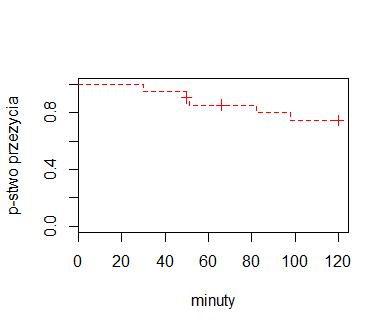
\includegraphics[width=0.5\textwidth]{1.png}
\end{figure}

\begin{knitrout}
\definecolor{shadecolor}{rgb}{0.969, 0.969, 0.969}\color{fgcolor}\begin{kframe}
\begin{alltt}
\hlcom{# dla obu eksperymentow:}

\hlstd{sea.KM} \hlkwb{<-} \hlkwd{survfit}\hlstd{(}\hlkwd{Surv}\hlstd{(time, vomit)} \hlopt{~} \hlstd{intens,} \hlkwc{data} \hlstd{= seasick,} \hlkwc{conf.type} \hlstd{=} \hlstr{"none"}\hlstd{)}
\hlkwd{summary}\hlstd{(sea.KM)}

\hlkwd{plot}\hlstd{(sea.KM,} \hlkwc{col} \hlstd{=} \hlkwd{c}\hlstd{(}\hlstr{"red"}\hlstd{,} \hlstr{"blue"}\hlstd{),} \hlkwc{lty} \hlstd{=} \hlkwd{c}\hlstd{(}\hlnum{1}\hlstd{,} \hlnum{2}\hlstd{),} \hlkwc{xlab} \hlstd{=} \hlstr{"minuty"}\hlstd{,} \hlkwc{ylab} \hlstd{=} \hlstr{"p-stwo przezycia"}\hlstd{)}
\hlkwd{legend}\hlstd{(}\hlnum{5}\hlstd{,} \hlnum{0.3}\hlstd{,} \hlkwd{c}\hlstd{(}\hlstr{"pierwsze dosw."}\hlstd{,} \hlstr{"drugie dosw."}\hlstd{),} \hlkwc{col} \hlstd{=} \hlkwd{c}\hlstd{(}\hlstr{"red"}\hlstd{,} \hlstr{"blue"}\hlstd{),}
    \hlkwc{lty} \hlstd{=} \hlkwd{c}\hlstd{(}\hlnum{1}\hlstd{,} \hlnum{2}\hlstd{),} \hlkwc{cex} \hlstd{=} \hlnum{0.7}\hlstd{)}
\end{alltt}
\end{kframe}
\end{knitrout}


\begin{figure}[h]
\centering
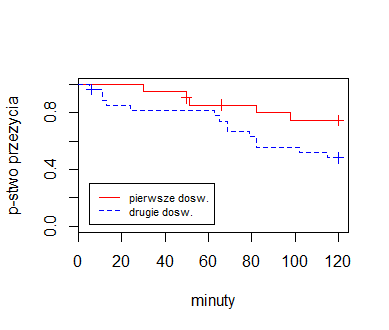
\includegraphics[width=0.5\textwidth]{2.png}
\end{figure}

\begin{knitrout}
\definecolor{shadecolor}{rgb}{0.969, 0.969, 0.969}\color{fgcolor}\begin{kframe}
\begin{alltt}
\hlcom{# porowynywanie krzywych przezycia:}

\hlstd{sea.test} \hlkwb{<-} \hlkwd{survdiff}\hlstd{(}\hlkwd{Surv}\hlstd{(time, vomit)} \hlopt{~} \hlstd{intens,} \hlkwc{data} \hlstd{= seasick,} \hlkwc{rho} \hlstd{=} \hlnum{0}\hlstd{)}
\hlstd{sea.test}
\end{alltt}
\begin{verbatim}
## Call:
## survdiff(formula = Surv(time, vomit) ~ intens, data = seasick, 
##     rho = 0)
## 
##           N Observed Expected (O-E)^2/E (O-E)^2/V
## intens=1 21        5     8.86      1.68      3.21
## intens=2 28       14    10.14      1.47      3.21
## 
##  Chisq= 3.2  on 1 degrees of freedom, p= 0.0733
\end{verbatim}
\begin{alltt}
\hlcom{# p-value duze, zatem przyjmujemy hipoteze, czyli krzywe przezycia nie}
\hlcom{# roznia sie istotnie}
\end{alltt}
\end{kframe}
\end{knitrout}


\subsection*{\textbf{\underline{Zadanie 2.}}}

\begin{knitrout}
\definecolor{shadecolor}{rgb}{0.969, 0.969, 0.969}\color{fgcolor}\begin{kframe}
\begin{alltt}
\hlstd{nsclc} \hlkwb{<-} \hlkwd{read.dta}\hlstd{(}\hlstr{"C:\textbackslash{}\textbackslash{}Users\textbackslash{}\textbackslash{}Marta\textbackslash{}\textbackslash{}Desktop\textbackslash{}\textbackslash{}Marta\textbackslash{}\textbackslash{}studia\textbackslash{}\textbackslash{}rok4\textbackslash{}\textbackslash{}Biostatystyka\textbackslash{}\textbackslash{}1\textbackslash{}\textbackslash{}nsclc_eng.dta"}\hlstd{)}
\hlkwd{head}\hlstd{(nsclc)}
\end{alltt}
\begin{verbatim}
##   patient mutation survtime survind tnm expression
## 1       1        1    24.51       1   2          1
## 2       2        1    27.13       1   2          1
## 3       3        0    34.84       0   2          1
## 4       4        1    35.70       0   2          1
## 5       5        1    27.90       0   3          1
## 6       6        1    25.67       0   3          1
\end{verbatim}
\end{kframe}
\end{knitrout}


\begin{knitrout}
\definecolor{shadecolor}{rgb}{0.969, 0.969, 0.969}\color{fgcolor}\begin{kframe}
\begin{alltt}
\hlstd{nsclc.KM} \hlkwb{<-} \hlkwd{survfit}\hlstd{(}\hlkwd{Surv}\hlstd{(survtime, survind)} \hlopt{~} \hlstd{expression,} \hlkwc{data} \hlstd{= nsclc,} \hlkwc{conf.type} \hlstd{=} \hlstr{"none"}\hlstd{)}

\hlkwd{plot}\hlstd{(nsclc.KM,} \hlkwc{col} \hlstd{=} \hlkwd{c}\hlstd{(}\hlstr{"red"}\hlstd{,} \hlstr{"blue"}\hlstd{),} \hlkwc{lty} \hlstd{=} \hlkwd{c}\hlstd{(}\hlnum{1}\hlstd{,} \hlnum{2}\hlstd{),} \hlkwc{xlab} \hlstd{=} \hlstr{"miesiace"}\hlstd{,} \hlkwc{ylab} \hlstd{=} \hlstr{"p-stwo przezycia"}\hlstd{)}
\hlkwd{legend}\hlstd{(}\hlnum{0.4}\hlstd{,} \hlnum{0.3}\hlstd{,} \hlkwd{c}\hlstd{(}\hlstr{"brak ekspresji bialka"}\hlstd{,} \hlstr{"ekspresja bialka"}\hlstd{),} \hlkwc{col} \hlstd{=} \hlkwd{c}\hlstd{(}\hlstr{"red"}\hlstd{,}
    \hlstr{"blue"}\hlstd{),} \hlkwc{lty} \hlstd{=} \hlkwd{c}\hlstd{(}\hlnum{1}\hlstd{,} \hlnum{2}\hlstd{),} \hlkwc{cex} \hlstd{=} \hlnum{0.7}\hlstd{)}
\end{alltt}
\end{kframe}
\end{knitrout}


\begin{figure}[h]
\centering
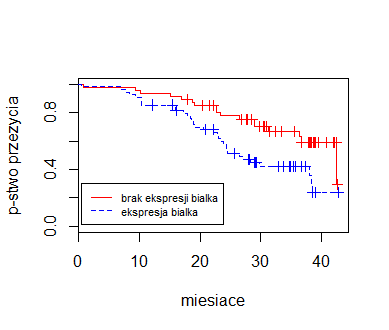
\includegraphics[width=0.5\textwidth]{3.png}
\end{figure}

\begin{knitrout}
\definecolor{shadecolor}{rgb}{0.969, 0.969, 0.969}\color{fgcolor}\begin{kframe}
\begin{alltt}
\hlstd{nsclc.test} \hlkwb{<-} \hlkwd{survdiff}\hlstd{(}\hlkwd{Surv}\hlstd{(survtime, survind)} \hlopt{~} \hlstd{expression,} \hlkwc{data} \hlstd{= nsclc)}
\hlstd{nsclc.test}  \hlcom{# krzywe roznia sie istotnie}
\end{alltt}
\begin{verbatim}
## Call:
## survdiff(formula = Surv(survtime, survind) ~ expression, data = nsclc)
## 
##               N Observed Expected (O-E)^2/E (O-E)^2/V
## expression=0 47       17     26.2      3.25      7.11
## expression=1 55       32     22.8      3.75      7.11
## 
##  Chisq= 7.1  on 1 degrees of freedom, p= 0.00769
\end{verbatim}
\begin{alltt}
\hlcom{# test warstwowy:}

\hlstd{nsclc.test.w} \hlkwb{<-} \hlkwd{survdiff}\hlstd{(}\hlkwd{Surv}\hlstd{(survtime, survind)} \hlopt{~} \hlstd{expression} \hlopt{+} \hlkwd{strata}\hlstd{(tnm),}
    \hlkwc{data} \hlstd{= nsclc)}
\hlstd{nsclc.test.w}
\end{alltt}
\begin{verbatim}
## Call:
## survdiff(formula = Surv(survtime, survind) ~ expression + strata(tnm), 
##     data = nsclc)
## 
##               N Observed Expected (O-E)^2/E (O-E)^2/V
## expression=0 47       17     25.5      2.82      6.05
## expression=1 55       32     23.5      3.06      6.05
## 
##  Chisq= 6.1  on 1 degrees of freedom, p= 0.0139
\end{verbatim}
\end{kframe}
\end{knitrout}


\begin{knitrout}
\definecolor{shadecolor}{rgb}{0.969, 0.969, 0.969}\color{fgcolor}\begin{kframe}
\begin{alltt}
\hlcom{# wykresy dla warstw oddzielnie:}

\hlstd{nsclc.KM.1} \hlkwb{<-} \hlkwd{survfit}\hlstd{(}\hlkwd{Surv}\hlstd{(survtime, survind)} \hlopt{~} \hlstd{expression,} \hlkwc{data} \hlstd{= nsclc,} \hlkwc{conf.type} \hlstd{=} \hlstr{"none"}\hlstd{,}
    \hlkwc{subset} \hlstd{= tnm} \hlopt{==} \hlnum{1}\hlstd{)}
\hlkwd{plot}\hlstd{(nsclc.KM.1,} \hlkwc{col} \hlstd{=} \hlkwd{c}\hlstd{(}\hlstr{"red"}\hlstd{,} \hlstr{"blue"}\hlstd{),} \hlkwc{lty} \hlstd{=} \hlkwd{c}\hlstd{(}\hlnum{1}\hlstd{,} \hlnum{2}\hlstd{),} \hlkwc{xlab} \hlstd{=} \hlstr{"miesiace"}\hlstd{,} \hlkwc{ylab} \hlstd{=} \hlstr{"p-stwo przezycia"}\hlstd{,}
    \hlkwc{main} \hlstd{=} \hlstr{"TNM = 1"}\hlstd{)}
\hlkwd{legend}\hlstd{(}\hlnum{0.4}\hlstd{,} \hlnum{0.3}\hlstd{,} \hlkwd{c}\hlstd{(}\hlstr{"brak ekspresji bialka"}\hlstd{,} \hlstr{"ekspresja bialka"}\hlstd{),} \hlkwc{col} \hlstd{=} \hlkwd{c}\hlstd{(}\hlstr{"red"}\hlstd{,}
    \hlstr{"blue"}\hlstd{),} \hlkwc{lty} \hlstd{=} \hlkwd{c}\hlstd{(}\hlnum{1}\hlstd{,} \hlnum{2}\hlstd{),} \hlkwc{cex} \hlstd{=} \hlnum{0.7}\hlstd{)}
\hlstd{nsclc.KM.2} \hlkwb{<-} \hlkwd{survfit}\hlstd{(}\hlkwd{Surv}\hlstd{(survtime, survind)} \hlopt{~} \hlstd{expression,} \hlkwc{data} \hlstd{= nsclc,} \hlkwc{conf.type} \hlstd{=} \hlstr{"none"}\hlstd{,}
    \hlkwc{subset} \hlstd{= tnm} \hlopt{==} \hlnum{2}\hlstd{)}
\hlkwd{plot}\hlstd{(nsclc.KM.2,} \hlkwc{col} \hlstd{=} \hlkwd{c}\hlstd{(}\hlstr{"red"}\hlstd{,} \hlstr{"blue"}\hlstd{),} \hlkwc{lty} \hlstd{=} \hlkwd{c}\hlstd{(}\hlnum{1}\hlstd{,} \hlnum{2}\hlstd{),} \hlkwc{xlab} \hlstd{=} \hlstr{"miesiace"}\hlstd{,} \hlkwc{ylab} \hlstd{=} \hlstr{"p-stwo przezycia"}\hlstd{,}
    \hlkwc{main} \hlstd{=} \hlstr{"TNM = 2"}\hlstd{)}
\hlkwd{legend}\hlstd{(}\hlnum{0.4}\hlstd{,} \hlnum{0.3}\hlstd{,} \hlkwd{c}\hlstd{(}\hlstr{"brak ekspresji bialka"}\hlstd{,} \hlstr{"ekspresja bialka"}\hlstd{),} \hlkwc{col} \hlstd{=} \hlkwd{c}\hlstd{(}\hlstr{"red"}\hlstd{,}
    \hlstr{"blue"}\hlstd{),} \hlkwc{lty} \hlstd{=} \hlkwd{c}\hlstd{(}\hlnum{1}\hlstd{,} \hlnum{2}\hlstd{),} \hlkwc{cex} \hlstd{=} \hlnum{0.7}\hlstd{)}
\hlstd{nsclc.KM.3} \hlkwb{<-} \hlkwd{survfit}\hlstd{(}\hlkwd{Surv}\hlstd{(survtime, survind)} \hlopt{~} \hlstd{expression,} \hlkwc{data} \hlstd{= nsclc,} \hlkwc{conf.type} \hlstd{=} \hlstr{"none"}\hlstd{,}
    \hlkwc{subset} \hlstd{= tnm} \hlopt{==} \hlnum{3}\hlstd{)}
\hlkwd{plot}\hlstd{(nsclc.KM.3,} \hlkwc{col} \hlstd{=} \hlkwd{c}\hlstd{(}\hlstr{"red"}\hlstd{,} \hlstr{"blue"}\hlstd{),} \hlkwc{lty} \hlstd{=} \hlkwd{c}\hlstd{(}\hlnum{1}\hlstd{,} \hlnum{2}\hlstd{),} \hlkwc{xlab} \hlstd{=} \hlstr{"miesiace"}\hlstd{,} \hlkwc{ylab} \hlstd{=} \hlstr{"p-stwo przezycia"}\hlstd{,}
    \hlkwc{main} \hlstd{=} \hlstr{"TNM = 3"}\hlstd{)}
\hlkwd{legend}\hlstd{(}\hlnum{0.4}\hlstd{,} \hlnum{0.3}\hlstd{,} \hlkwd{c}\hlstd{(}\hlstr{"brak ekspresji bia�ka"}\hlstd{,} \hlstr{"ekspresja bialka"}\hlstd{),} \hlkwc{col} \hlstd{=} \hlkwd{c}\hlstd{(}\hlstr{"red"}\hlstd{,}
    \hlstr{"blue"}\hlstd{),} \hlkwc{lty} \hlstd{=} \hlkwd{c}\hlstd{(}\hlnum{1}\hlstd{,} \hlnum{2}\hlstd{),} \hlkwc{cex} \hlstd{=} \hlnum{0.7}\hlstd{)}
\end{alltt}
\end{kframe}
\end{knitrout}


\begin{figure}[h]
\begin{minipage}[t]{0.5\textwidth}
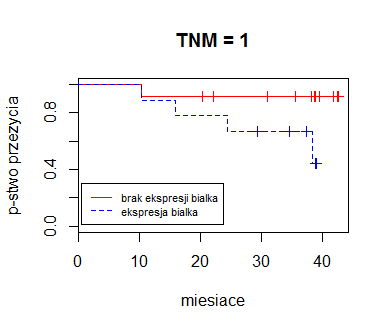
\includegraphics[width=\textwidth]{4.png}
\end{minipage}
\begin{minipage}[t]{0.5\textwidth}
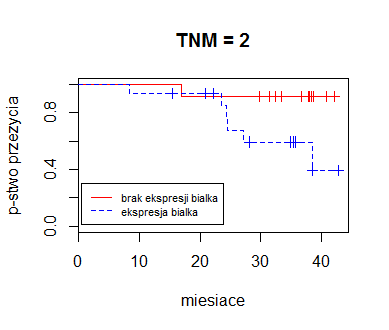
\includegraphics[width=\textwidth]{5.png}
\end{minipage}
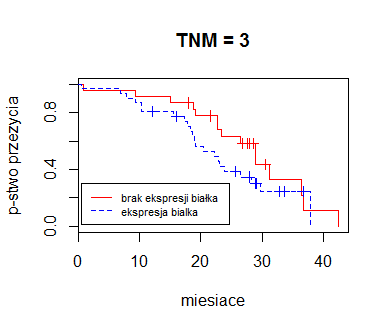
\includegraphics[width=0.5\textwidth]{6.png}
\end{figure}
\end{document}
